\section{Sector specific application of frameworks}

This paper is based on the organisation of the economy in specific industries. The International Standard Industrial Classification of All Economic Activities (\ac{ISIC}) provides a high level set of sections which are ultimately leading to particular industries. In this paper, we use a consolidated version of those 21 sections which result in 11 groups, which are stated out below: \cite[p.271, table 4]{ISIC:2008}

\begin{enumerate}
\item Agriculture, forestry and fishing [ISIC: A]
\item Manufacturing [ISIC: C]
\item Mining and quarrying; Electricity, gas, water supply and other industrial activities [ISIC: B,D,E]
\item Construction [ISIC: F]
\item Wholesale and retail trade, transportation and storage, accommodation and food service activities [ISIC: G,H,I]
\item Information and Communication [ISIC: J]
\item Financial and Insurance activities [ISIC: K]
\item Real estate activities [ISIC: L]
\item Professional, scientific, technical, administrative and support service activities [ISIC: M, N]
\item Public administration and defence, education, human health and social work activities [ISIC: O,P,Q]
\item Other service activities [ISIC: R,S,T,U]
\end{enumerate}

\subsection{Agriculture, forestry and fishing}
%JO
%Literatur Angaben  1) Internet of Food and Farm 2020
%                   2) http://www.bauernverband.de/36-digitalisierung-in-der-landwirtschaft

The agricultural section is highly influenced by \ac{I4.0} innovations. Examples are smart agriculture, smart farming, vertical and horizontal integration of the supply chain to provide sustainable food chains and automated processes to deliver high-quality food. Farms and food companies are increasingly developing towards high-tech factories and large-scale production, intensively relying on digital technology. \cite[p.129-151]{FoodAndFarm2020} \ac{IoT} technologies and sensors are used to monitor agricultural status and development by enabling digital tracking and tracing processes to provide food safety, quality management, optimize food production and manufacturing. Growing consumer claims concerning food quality and food availability are pushing the agricultural sector forward. \cite[p.131]{FoodAndFarm2020}.


\begin{figure}[H]
\centering
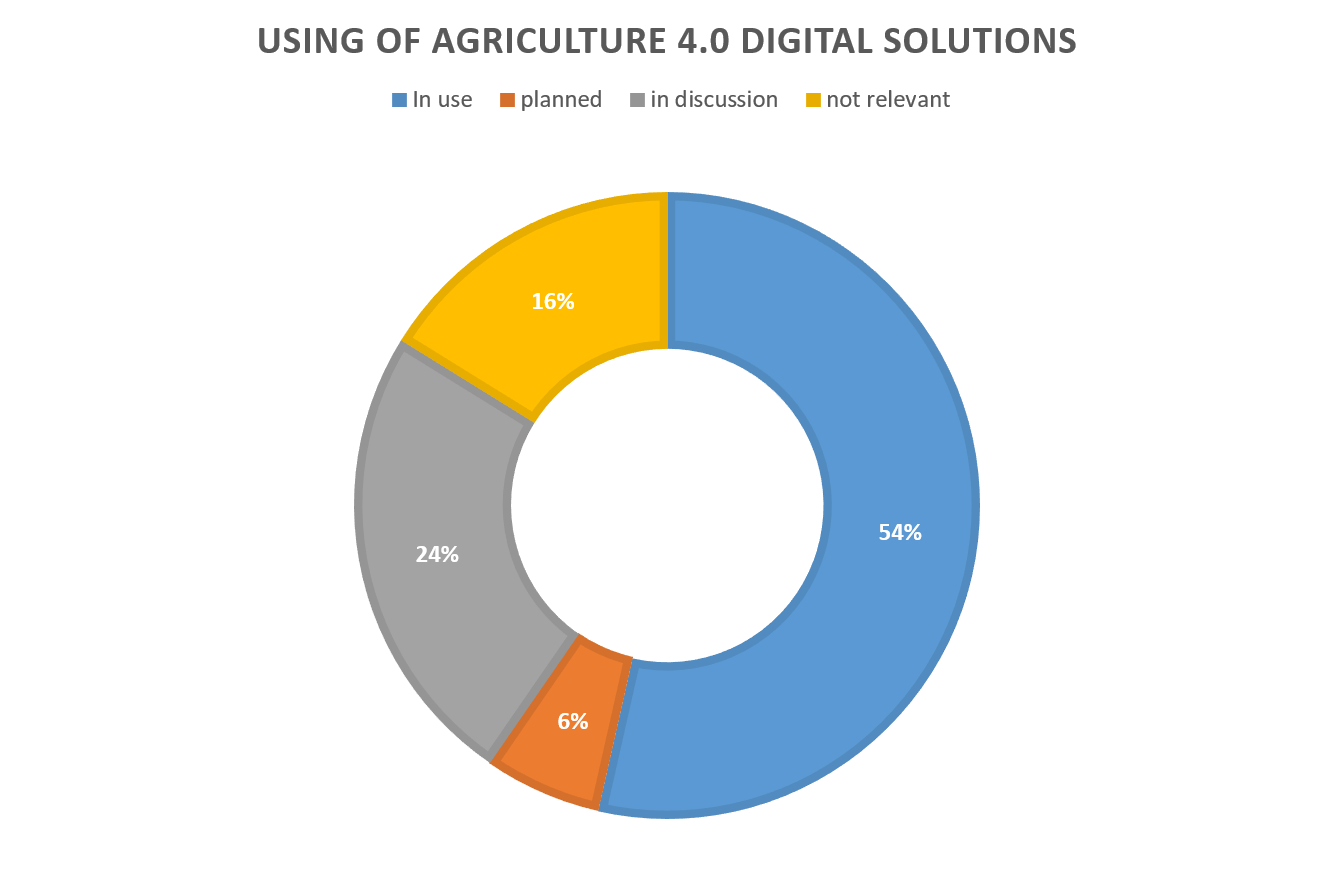
\includegraphics[width=1\columnwidth]{images/usingOfAgriculure4-0-solutions_pieChart}
\caption{Using of Agriculture 4.0 digital solutions \cite{digitAgrad}}
\end{figure}


To get an initial impression of the \ac{IoT} progress and level of digitalization in the agriculture industry, the figure above states out how many german companies in that industry are using and/or planning to use \ac{IoT} and digital solutions to optimize their agricultural business \cite{digitAgrad}.

In general, smart farming and the use of \ac{IoT} technologies are increasing crop yields. Precise data about utilised agricultural area, weather and realtime tracking of active machines and systems are leading to higher food quality and more efficient use of ressources.

Challenges of the agriculture, forestry and fishing sector are linked to the ecological/climate change regarding consumer concerns and the globally increasing demand of food. \ac{I4.0} concepts are used to face those challenges.


\begin{figure}[H]
\centering
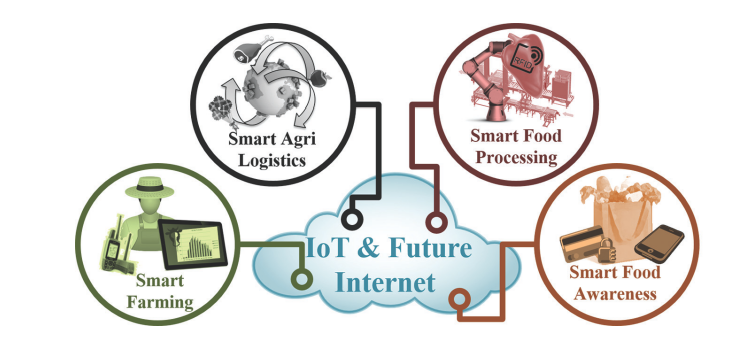
\includegraphics[width=1\columnwidth]{images/digitising-industry_agriculture_smartFarming}
\caption{Domains which are impacting the industry from \cite[p.133]{FoodAndFarm2020}}
\end{figure}


Domains like smart farming, smart Agri-logistics, smart food processing and smart food awareness are used to describe the development of \ac{IoT} impact on the sector \cite[p.133]{FoodAndFarm2020}.

The \ac{RAMI}, goals and guidelines of the \ac{I4.0} and \ac{IIC} initiatives can be applied at a general/strategic level in the Agriculture, forestry and fishing industry. It is important to determine technical standards and platforms to get \ac{IoT} and digital solutions connected with customary activities in that industry. Nevertheless, it is important to gather industry-specific information on how to get \ac{IoT} implemented in business processes.
The following frameworks can deliver more specific guidelines for the agriculture, fishing and forestry industry:

\begin{itemize}
\item The PRECOS framework linked with \ac{IoT} technology \cite{Trolard2016590}
\item SmartFarmNet \ac{IoT} platform \cite{InternetOfThingsAgricultureSmartFarming}
\item Virtualized Food supply chains \cite{Verdouw2016128}
\end{itemize}


\subsection{Manufacturing}
The manufacturing sector is the most discussed sector in the literature. It is the focus sector of the \ac{I4.0} initiative and many companies such as McKinsey actually see \ac{I4.0} as a synonym for the digitalization of the manufacturing sector \cite[]{McKinseydigitizationIndustrialSector:2015}. Little beneficial advise can be given by us for this sector as it is being focused on by the \ac{I4.0} initiative itself and the suggestion should therefore be to follow this frameworks approaches as well as the \ac{IIC} publications regarding the cross sector specific interests \cite[]{iicarchitecture:2016}.

\subsection{Mining and quarrying; Electricity, gas, water supply and other industrial activities }

The sector of supplying basic utilities such as electricity, gas and water is a complex system in each vertical and horizontal level. Each level brings with it potentials and problems, but a generalized description is the task of finding a transportable base resource, extracting and delivering it to end consumers. The sector therefore requires extraction activities, industrial processing capabilities, supply chains and the \emph{"operation of transmission [and] distribution systems"}\cite[p. 166ff]{ISIC:2008} for various utilities such as gas, electricity, water and others.

The electricity grid especially has been a focus of studies due to the politically demanded changes in energy sources and delivery \cite[p.12ff]{AppelrathKagermannMayer2012}. Regarding the delivery of products that are not using a continuous delivery network such as the electricity or water supply grid, the recommendations by the \ac{WEF} can be applied that focus on logistics' improvement of efficiency and describe a \emph{"race to build a dominant global [logistics] platform"}\cite{worldforumlogistics:2016}. Regarding the industrial processing capabilities, again the \acf{I4.0Init} offers many guidelines and best practices.

The extraction of minerals in the form of mining and quarrying have been the focus by \citeauthor{mckinseymining:2015} who describe mining as a sector that has suffered from decreasing profitability due to a continuous price competition and competitors continuously improving their productivity. They imply that mining can greatly benefit from the classic building blocks of digitalization such as increased precision through sensors and downstream analytics to improve \emph{"material and equipment flow"} and create a \emph{"deeper understanding of the resource base"}. Automation, robotics and analytics can help improve efficiency and reduce downtime. Big improvement potentials become obvious when we look at the amount of data used for decision making which is a meager 1\% of the total data collected \cite[p.7]{mckinseymining:2015}.

Literature suggestions, aside from the works of the \ac{IIC} and \ac{I4.0Init} are therefore:

\begin{itemize}
\item Digital Transformation of Industries: Logistics \cite{worldforumlogistics:2016}
\item How digital innovation can improve mining productivity \cite{mckinseymining:2015}
\item Future Energy Grid: Migrationspfade ins Internet der Energie \cite{AppelrathKagermannMayer2012}
\end{itemize}


\subsection{Construction}
%JO
%Quelle: Digitalisierung der Bauwirtschaft, Der europäische Weg zu "Construction 4.0", Roland Berger, 2016
%Quelle: Towards the next generation of intelligent building, Geriogius Lilis
%Quelle: Big Data in the construction industry, Muhammed Bilal
%Quelle: http://buildingsmart.org/about/vision-mission/core-purpose/

%TODO: Literaturangaben scannen

According to a poll of the german chamber of Industry and Commerce (\ac{DIHK}) on March 2016 \cite[]{barometer:2016}, the sample of companies linked to the construction and building industry rate their level of Digitalization on a scale from 1 to 6 as a 3.5, which is 0.2 points less than the average across all industries.\cite[p.5]{barometer:2016} This states out, that representatives of the construction industry know, that they generate advantages, when they use digital solutions and \ac{IoT} \cite[p.7-8]{barometer:2016}, but are not implementing those fast enough.

The \ac{IoT} impact on the construction or building industry is linked to terms like smart cities, lean construction management and smart resource management in construction processes. The main focus of digitalization processes in this domain is to reach higher levels of sustainability and energy efficiency \cite{Lilis2017473}.
Intelligent buildings are the transformational core in this industry. Regarding development in this industry facing the smart city topic, \ac{IoT} is very important and a leading driving force impacting the progress in development. Lean construction management and smart resource management is linked to more traditional construction progresses, so generally \ac{IoT} is used to expand innovation in those areas and is not transforming it itself.

Current examples of digital tools which support processes like planning, analysing, monitoring, and optimizing the construction of objects are e.g. the Building Information Modeling (\ac{BIM}) and also building automation systems (\ac{BAS}) which served the purpose reliably in the previous decades but need to be transformed to models, which cover \ac{IoT} progress and technological standards throughout integrating industries and operations \cite{Lilis2017473}.

The \ac{BIM} and specifically the roadmap for digital Design and Construction \cite{FederalMinRoadMapConstruction}
are frameworks, which can be used to get digital processes involved in the industry regarding holistic perspectives or progress. To get this in connection to the current impact of the digitalization on the industry, the Federal Ministry of Transport and Digital Infrastructre makes the use of BIM mandatory for public infrastructural projects.\cite{FederalMinRoadMapConstruction}

\ac{BAS} and building management systems \ac{BMS} are used to integrate many different data resources and construction processes to offer an \emph{"economy of large scale with expertise in the system control and automation engineering domains"} \cite[p.475]{Lilis2017473} %TODO Quote formation check
This states out, that these systems are being developed and are facing the challenges of \ac{I4.0}. On the other hand, the industries' best practices are legacy habits with small innovation progress e.g. because of the close relationship to the public administration sector and administrative barriers \cite{Oesterreich2016121}

In this paper, we can only state out general information about specific models, but the initiative \emph{"building smart"} \cite{buildingsmart:2016} %TODO Literaturangabe checken
and their so-called \emph{"international home of openBMI"} is recommended to get further information regarding the assessment and status of \ac{I4.0} progress in construction or building-industry focused businesses. Additionally, we can recommend the \emph{BIMiD reference construction process}, which delivers an example of digitally planned construction project \cite{bimidReferencemodel:2016} % TODO Link check

\begin{figure}[H]
\centering
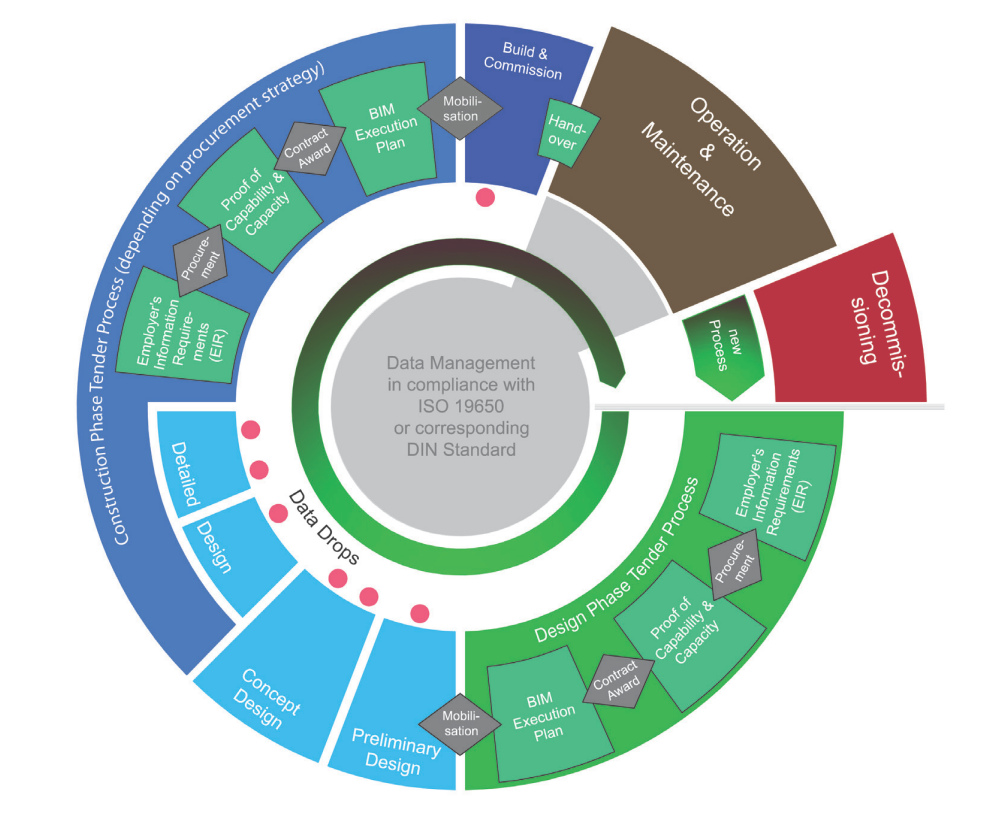
\includegraphics[width=1\columnwidth]{images/construction-BIM-reference-process.PNG}
\caption{Schematic illustration of the BIM reference process from \cite{FederalMinRoadMapConstruction}}
\end{figure}

To sum up, the construction industry can get general guidelines to transform operations and processes, culture and business models using the frameworks introduced in chapter~\ref{subsec:frameworks}. This can be applied to generate strategic transformation in the industry and the core goals of \ac{I4.0} are analogous to the construction-industry specific ones. Profound effects or viable addition can get achieved by applying the described models \ac{BIM}, \ac{BAS}, and guidelines by industry-focussed initiatives.

\subsection{Wholesale and retail trade, transportation and storage, accommodation and food service activities}

This group is a collection of three sectors defined by \ac{ISIC}. The first sector, wholesale and retail trade, includes all \emph{"services incidental to the sale of [...] goods"}\cite[p.179]{ISIC:2008} as well as the specific task of motor vehicle repairs. The second sector, transportation and storage, includes all tasks related to logistics and storage of both objects and passengers.\cite[p.194]{ISIC:2008} The last one is focusing on the \emph{"short-stay accommodation for visitors"} as well as the \emph{"provision of complete meals and drinks fit for immediate consumption"}\cite[p.202]{ISIC:2008}

%TODO PB wholesale
Wholesale and Retail have seen high efficiency improvements through integrated supply chain systems with suppliers, sensor based indoor navigation and improved customer experiences with on-the-fly cashier systems \cite{tescoretail:2015, iicretailbrick:2016} by large chains like Tesco. On the other side of the spectrum, small and medium size businesses found their opportunities in niche markets, playing on their strength of agility and ability to quickly innovate to answer changing consumer demands \cite{pwcretailrenaissance:2016}. This section is a perfect example of the two sides of \ac{DT}: Rapid efficiency increases challenging competitors prices and diverse business models adapting to changing customer demands and creating new markets. 

The second section, transportation and storage, often also called logistics, offers large optimization potentials. As reported by \citeauthor{nytimesdrivingtruck:2016} in the New York Times, Uber, a digital pioneer in on-demand drive-hauling services, is actively working on autonomous trucks for logistics which has been demonstrated by an autonomously driving truck transporting goods 120 miles without the need of a driver in October 2016. Amazon recently introduced "intelligent" robots in their warehouses, greatly reducing the walking distances of "pickers", employees who collect products for orders. \cite{Kiva:amazon:Ma:2016:OTA:2936924.2937092}. Drones are being investigated as alternatives for delivering parcels and analytics can help fill many of empty trucks that can be up to 50\% of a fleet on their return trips \cite{worldforumlogistics:2016}.

The third sector, accommodation and food service activities, has already seen its fair share of digitalization fueled disruption with AirBnB disrupting the accommodation market and companies like foodora and deliveroo offering services aim to remove the location component of food services \cite{bloombergfoodora:2016}. Both are strategic markets that can be expected to stay, as long as humans eat, travel and sleep, but the model of serving these demands can differ greatly from current business models. Existing businesses need to challenge their business models and be willing to disrupt their own business to avoid competition from doing so.

For all three sectors in this group, the recommendations of the \ac{IIC} and \ac{I4.0Init} are valid. Especially the \ac{IIC} recommendations regarding vertical integrations of value chains in their architectural recommendations \cite{iicarchitecture:2016} are valuable for all three sectors due to their direct link with supply chains and logistic companies. In addition the following literature recommendations can be made:

\begin{itemize}
    \item The Business Model Navigator: 55 Models That Will Revolutionise Your Business \cite{gassmann:gallen:2013geschaeftsmodelle}
    \item Leading Digital \cite{bonnect2014leading}
    \item World Economic Forum White Paper Digital Transformation of Industries: Logistics Industry \cite{worldforumlogistics:2016}
\end{itemize}

\subsection{Information and Communication}
Included in the information and communication section is, next to information technology and software, which are some of the main drivers of the digitalization, also publishing, motion picture and sound recording activities. These industries have seen what digitalization and disruption means in several cases, ranging from online music and movie streaming services like Spotify and Netflix to more distributed yet still substantial changes such as online publishing and blogging. Blogs and social networks have shifted consumer expectations and challenged established companies such as newspapers and magazines that quickly had trouble competing with these free alternatives which solely relied on advertisement for financing themselves and which had enjoyed much stronger network effects than traditional publishing. 

Overall it can be summarized that this section struggles with disrupting new entrants to the market that challenge existing business models with new, digital alternatives. Businesses should therefore focus their efforts on reevaluating their business model as well as their culture with the frameworks provided in chapter~\ref{subsec:frameworks}. Regarding the information technology and software development industries, advise will be given in chapter~\ref{subsec:profscience}. 

\subsection{Financial and insurance activities}
%JO
%TODO Literaturangaben scannen

The financial services industry, including financial service activities, Insurance, reinsurance, pension funding and activities auxiliary to Financial and insurance activities \citeauthor{ISIC:2008} are facing transformation throughout digitalization processes. The final Report of the \ac{WEF} addresses the future of financial services regarding the impact of disruptive innovations and \ac{IoT} \cite{WEF-futureFinancialServices} and is dividing the financial services industry into 6 functions and 11 Clusters of Innovation \cite{WEF-futureFinancialServices}, which are influencing and are influenced by disruptive innovations and digitalization progress.
The functions are:
Payments, Insurance, Deposits \& Lending, Capital Raising, Investment Management, Market Provisioning

The clusters of Innovation are:
Emerging Payment Rails, Cashless World, Insurance Disaggregation, Connected Insurance, Alternative Lending, Shifting Customer Preferences, Crowdfunding, Empowered Investors, Process Externalisation, New Market Platforms, Smarter \& faster Machines.

Furthermore, the progress in several functions is currently shaping new business opportunities, e.g. fintech start-ups or more integrated business processes which are generating more values for the economy and the requirements of the society.
Typical barriers of the industry and the implementation of innovations like \ac{IoT} are Accountability, Privacy, Security, Interoperability and Reliability. \cite{WEF-futureFinancialServices, Weber2011133, CapGemini-IoT-financialServices} %TODO Literaturhinweis überprüfen

The pressure of innovating legacy processes in this industry is already latent. To get profound results, the transformation requires changes in areas, which are linked to each other. Therefore, integration is elementary for success. As it is stated out in the paper of \citeauthor{ArthurDLittle-FinancialService} \emph{"The transformation normally requires important changes in processes, organization structure, and company systems, and must involve all business and IT areas"} \cite[p.4 ]{ArthurDLittle-FinancialService}. Accenture's \emph{European Financial Services Digital Readiness Report} also confirms, that financial services firms need to change their processes all over the their organization across the four core business areas plan, make, sell and manage. \cite[p. 9]{accenture-europeanFinancialServices-digitalReadinessReport}

Regarding these profound changes in the financial and insurance activities, it has to be stated out, if the \ac{IIC} and \ac{I4.0} Frameworks can be applicable to accomplish the progress. The \ac{RAMI} itself is a good starting point for the financial services industry, but cannot outline specific challenges and conditions of that section. Extending those frameworks with the following, more detailed ones, is recommended:

\begin{enumerate}
\item Six themes touching multiple clusters of innovation across functions \cite{WEF-futureFinancialServices}
\item The DIGITAL framework by Arthur D. Little \cite[]{ArthurDLittle-FinancialService}
\item Digital Readiness Assessments Framework by Accenture Research \cite{accenture-europeanFinancialServices-digitalReadinessReport}
\end{enumerate}

The first is the described in the \ac{WEF} \cite{WEF-futureFinancialServices} Report about the future of financial services and their functions. The six important themes that lead to \ac{I4.0}-progress in financial and insurance activities are streamlined Infrastructure, automation of high-value Activities, reduced intermediation, the strategic role of Data, niche \& specialised products and customer Empowerment. Applying those themes may help the financial industry to implement the chances and potential of fast developing processes based on digitalization and \ac{IoT}.

The \emph{DIGITAL framework} by Arthur D. Little \cite[]{ArthurDLittle-FinancialService} presents the main goals of digitalization and their respective measurement \ac{KPI} in the financial services industry. It is structured in seven parts which are in succession building the word \emph{DIGITAL} \cite{ArthurDLittle-FinancialService}: development of new Products, incentivice sales to current clients, generate new clients, image: positioning as an digital company, transfer operations to digital channels, automation of operations, loyalty and churn of clients. The best long-term improvements are stated out in the digital Image and the Transfer of operations to digital channels \cite{ArthurDLittle-FinancialService}

Accenture Research developed a Digital Readiness Assessments Framework \cite{accenture-europeanFinancialServices-digitalReadinessReport}, which emphasizes that there is the need to change both inside and out. Therefore it is important to fill the gap between planning to get digital and fully merging the plan with the business reality. The framework can be seen as a strategic recommendation for decision-makers of the industry and is defining three key areas of change: Define - or redefine - the business, become integral to the online experience and Change the operating model \cite{accenture-europeanFinancialServices-digitalReadinessReport}. 

\subsection{Real estate activities}
%JO

Companies appurtenant to the real estate industry face several similar challenges like the construction industry.
The \ac{ISIC} defines two activity groups in this industry: Real estate activities with own or leased property \& Real estate activities on a fee or contract basis \cite{ISIC:2008}. Other activities, like the real-estate broker or property management can use \ac{IoT} to automate monitoring current status of real estate objects or energy supply on the spot. 

In this paper we suggest to use the recommended frameworks of the construction section, combined with the section \emph{Other service activities}. 

\subsection{Professional, scientific, technical, administrative and support service activities}
\label{subsec:profscience}

%PB

Professional services such as legal support, administration, engineering and architecture are affected very little by the effects of digitalization and industry 4.0 in the sense that they aren't the ones getting digitalised but rather are the ones pushing forward this transformation. It is therefore not logical to apply \ac{I4.0} concepts to this sector, however it is important for those professionals to be knowledgeable about the factors of it since they are major players regarding its planning and implementation. They should therefore have a broad high level knowledge about the overall trend with specialized knowledge for their focus industries.

In the phase of designing the \ac{DT} there are many relevant topics. Managing roles focus on the planning and controlling of the business branches and activities. Such tasks can greatly benefit from knowledge derived from the information exposed through sensors and analysed with tools from data science enabling \emph{"real-time business and operational decisions"} \cite[p.84]{iicarchitecture:2016}.

There are also big aspects such as security, governance and controlling activities that can benefit from the \ac{DT}. As \citeauthor{Tragos2016trusted} note, The \ac{IoT} leads to many unnoticeable devices spread around public places that monitor and log a variety of information which can be considered a necessary tool but also a source of privacy invasion. Strong security measures need to be deployed to ensure all dimensions of the \emph{\ac{IoT} trustworthiness} are covered which are explained in detail by the \ac{IIC} in their Security Framework \cite{iicsecurity:2016}.

\begin{figure}[H]
\centering
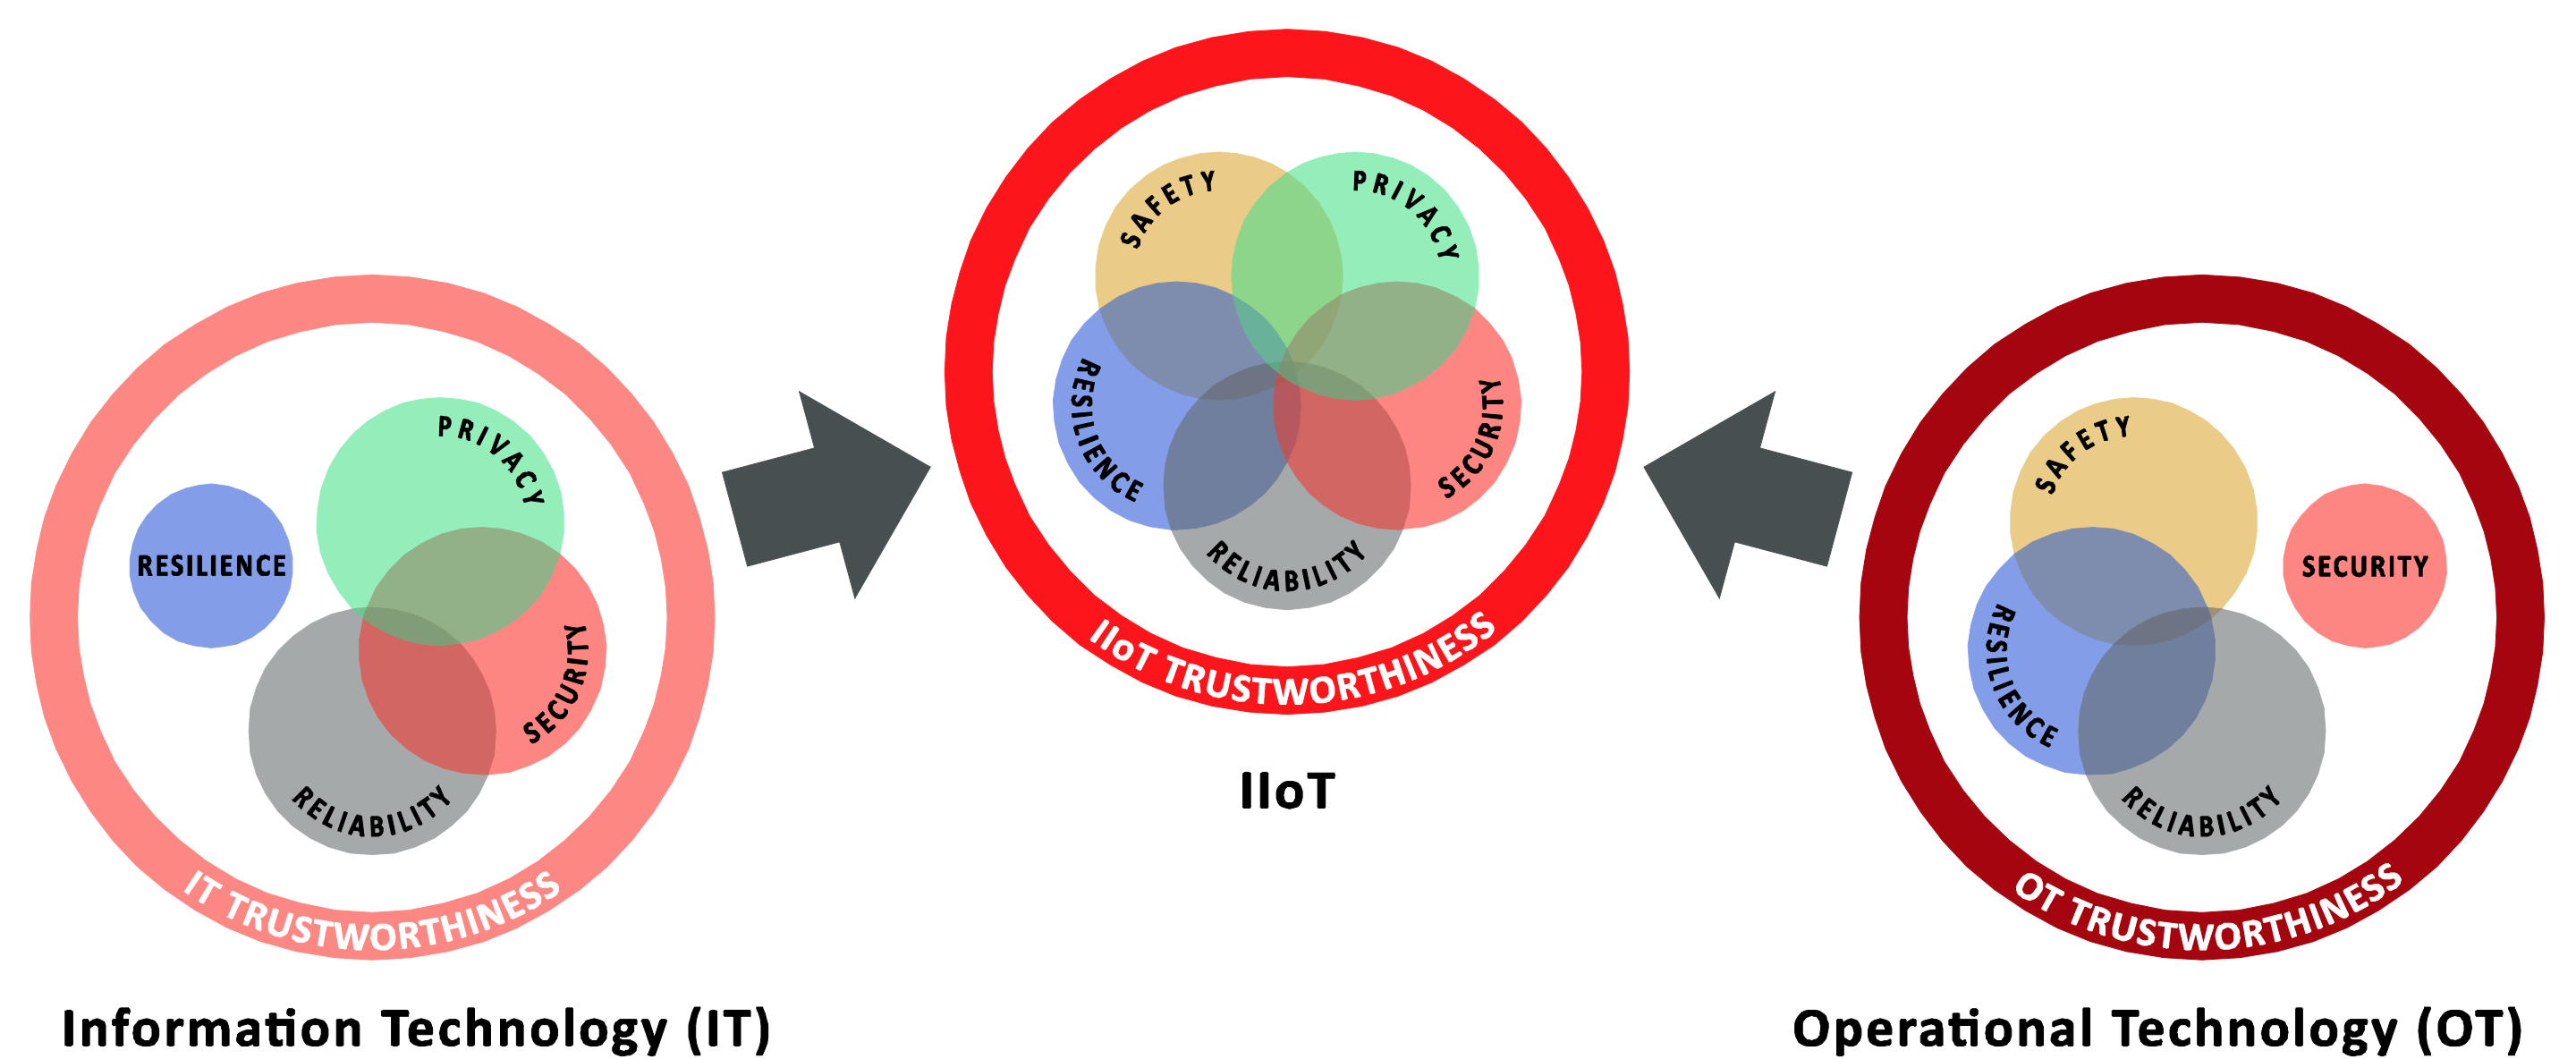
\includegraphics[width=1\columnwidth]{images/iic-iiot-trustworthiness}
\caption{\ac{IIC} Security Framework}
\end{figure}

To summarise, the sector is a major player in the design of the \ac{DT} but is not directly affected by it in the sense of it being the subject of transformation. Professionals and businesses in this sector are therefore advised to build up knowledge about the \ac{DT} and familiarise themselves with the core concepts of \ac{I4.0}. The two frameworks by the \ac{IIC} and the \ac{I4.0} initiative are an excellent guideline for this.

\subsection{Public administration and defence, education, human health and social work activities}

This group is a collection of  three  sectors  defined  by \ac{ISIC}. The first section "Public administration and defence; compulsory social security" \emph{"activities of a governmental nature, normally carried out by the public administration"}\cite[p.243]{ISIC:2008}. The second section focuses on all activities regarding education, independent of level or form of communication and includes public and private education. The third section covers all activities regarding health care, ranging from hospitals to residential care and even social work activities that aren't performed by health care professionals\cite[p.254ff]{ISIC:2008}.

%- Digitale Verwaltung (E-Administration), german initiative pushing towards making all services to citizens available online
The first section, public administration activities, is under high pressure from its citizens to supply digitally available services. The German government set in motion a set of laws directing all administrations to redesign their processes towards digitally available services for citizens, companies and other stakeholders \cite{verwaltung:2014}. Although these activities usually involve services rather than manufacturing, the security guidelines developed my the \ac{IIC} and \ac{I4.0Init} are elementary to this section. A government must uphold the highest standards of security, especially with personal and sensitive data of its citizens as well as with defence related activities. Culture and business models are less significant although innovation, even in the public sector, is becoming more important \cite{derivwhitehouse:2016}. 

%- arizona state university education, using big data for customised individual level timetables %http://www.nytimes.com/2012/07/22/education/edlife/colleges-awakening-to-the-opportunities-of-data-mining.html
The second section, education finds its best example in Arizona. The Arizona State University is considered a \emph{"hotbed of data-driven experiments"}\cite{asutimes:2012} and uses large scale data analytics to improve students college life and education efficiency. Timetables are customised for every student, micro feedback allows highly precise control over students learning progress which reduces overall drop out rates. The whole education section offers big opportunities in data analytics but many institutions in the public domain don't have the funding to initiate large scale projects for collecting and analyzing data as the Arizona State University. Many schools in Germany are struggling with much more basic requirements such as building and fire safety, totaling about \euro{}32 billion in accumulated required financial support to support basic requirements\cite{schulen:2015}. This opens opportunities for private education businesses like Udacity, offering online education for computer science topics offering nano-degrees that are accepted by many big companies instead of a tertiary education \cite{udacity:2016}.


%- health: lots of opportunities, customised data, high fidelity \cite{diabetis:2014}
The third section, human health and social work activities has also been influenced strongly by \ac{IoT} technologies and consumer grade health products. \citeauthor{YIN20163} found that many physicians as well as insurances started hooking into the variety of fitness trackers currently available on the market to develop higher precision treatment and insurance plans. \citeauthor{diabetis:2014}, a neuroscientist analyzed her sons diabetes with high precision tooling to better understand the disease but was shocked by her sons physician who could not make use of the data. The United States initiated the Open Data initiative aiming to provide large population scale data-sets for researchers to find answers for epidemics, education, energy problems and many other topics. 

For this group of sections we recommend the following literature, due to the heavy reliance on security concerns as well as data analytics potentials:
\begin{itemize}
    \item Interview with Dhanurjay Patil, white house chief data scientist of the Obama administration \cite{derivwhitehouse:2016}
    \item Security recommendations by \ac{IIC} and \ac{I4.0Init}
    \item Speech of \citeauthor{diabetis:2014} about high precision diabetes tracking \cite{diabetis:2014}
\end{itemize}


%PB TODO
%JO habe ein gutes Uebersicht Paper fuer dich gefunden. Siehe Dropbox Literatur Ordner #healthcare-industry

\subsection{Other service activities}
%JO
The \ac{ISIC} defines this section as a residual category including Arts, entertainment and recreation Activities; membership organizations, repair services for personal equipment as well as cleaning and beauty services \cite[p.262ff.]{ISIC:2008}.

These categories of economic activity, aside from the membership organizations, are composed mainly of \ac{SME}. Such businesses rarely have the capacity to compose a complex implementation of a digitalization strategy which causes the \ac{I4.0} and \ac{IIC} frameworks to be not suitable.

The limited resources of \ac{SME} are located in financial capital, expertise of the staff and the impact on the economic environment \cite{JSBM:JSBM341}. Therefore the investment in digital transformation or implementation of \ac{IoT} and digitalization processes are to a great extent blocked by the limited resources.

Other examples of the entertainment or arts industry may have the chance to utilize \ac{IoT} and can apply the \ac{I4.0} frameworks combined with \ac{IIC} guidelines.

This industry is unfrugal to encapsulate, so the more generic frameworks are recommended. Analogies to other frameworks of adjunct industries should be determined.